\documentclass[final,twocolumn,12pt]{elsarticle}

\usepackage{amsmath}
\usepackage{amssymb}
\usepackage{booktabs}
\usepackage{enumitem}
\usepackage{graphicx}
\usepackage{lineno}
\usepackage{microtype}
\usepackage{multirow}
\usepackage[section]{placeins}
\usepackage{xcolor}
\usepackage[hidelinks]{hyperref}
\usepackage[nameinlink,noabbrev]{cleveref}
\emergencystretch=2em

\journal{Automation in Construction}
\biboptions{sort&compress}
\modulolinenumbers[5]

\newcommand{\systemname}{ConstructionSceneReady}
\newcommand{\placeholder}[1]{\textcolor{gray}{\textit{#1}}}
\newcommand{\plannedfigure}[4]{%
  \fbox{%
    \parbox{0.94\linewidth}{%
      \vspace{1.5mm}%
      \centering
      \textbf{#2}\par\medskip
      \begin{minipage}{0.88\linewidth}
        \small #3\par\medskip
        \textit{Planned evidence: #4}
      \end{minipage}%
      \vspace{1.5mm}%
    }%
  }%
}

\begin{document}

\begin{frontmatter}

\title{ConstructionSceneReady: Evidence-grounded compilation and task-scene
validation for BIM-driven robotic assembly}

% Author identities are intentionally kept in title-page.tex.

\begin{abstract}
Robot-ready construction simulation requires more than converting building
geometry into a simulation format. This study asks which building information
actually supports a robotic construction task in simulation, and how its
absence, error, or imprecision changes task outcomes. We propose
\systemname, which compiles IFC source into task-activated multi-scale OpenUSD
scenes and validates the composed scene against an explicit construction
task-scene contract with evidence-bounded repair. On a frozen 105-case
fault-injection partition, the contract recovers all 141 expected findings
without false positives; whitelisted repair restores 97.1\% of scenes to
pristine equivalence and escalates the rest. Constraining a language-model
agent to the same whitelist preserves this reliability (96.8\% valid, zero
incorrect repairs in 525 episodes), while an unconstrained agent produces
validator-passing but incorrect scenes in 22.7\%. Paired humanoid insertion
episodes then measure the task consequence of each information family:
symbolic and referential defects are discretely fatal, interface clearance is
the most sensitive continuous property, and absolute member-pose errors are
absorbed by closed-loop perception. Crossing these outcomes with the contract
shows perfect specificity but limited sensitivity to sub-tolerance geometric
fidelity; we convert that blind spot into two contract rules verified on an
independent test set. Evidence comes from parameterized fixtures and one
fixed-base executor with a kinematic grasp scaffold; the conclusions are
structural---which information families are fatal, graded, or
self-correcting---rather than absolute performance claims.
\end{abstract}

\begin{keyword}
building information modeling \sep OpenUSD \sep construction robotics \sep
humanoid robot \sep simulation validation \sep agentic repair
\end{keyword}

\end{frontmatter}

\linenumbers

\section{Introduction}
\label{sec:introduction}

Robotic construction is increasingly planned from digital building
information, yet the model delivered by a designer and the world required by a
robot remain fundamentally different artefacts. An Industry Foundation Classes
(IFC) model describes intended components, spatial containment, materials, and
design relationships. A robot simulator instead requires collision geometry,
mass properties, physical constraints, task targets, and an explicit account of
which objects and geometric details are active. The difference is not resolved
by changing file formats. It is a change from a representation of what should
be built to a representation of what can be acted upon, under a particular
construction state and by a particular embodiment.

The problem becomes more pronounced at building scale. Navigation through a
floor or room can be evaluated with simplified walls, openings, and obstacles,
whereas placing a connection plate or inserting a pin depends on
millimetre-scale interface geometry. Loading every building object at
interaction-level fidelity is wasteful and can make collision checking and
physics simulation unnecessarily expensive. Retaining only coarse geometry is
equally problematic: it can conceal penetrations, reverse an insertion axis, or
turn an infeasible assembly into an apparently valid one. A useful robot world
must therefore change its working set and geometric fidelity with the task
without losing identity or relationships across scales.

Previous studies have established important parts of this information chain.
BIM-derived robot worlds and task-planning systems have been generated for
painting, prefabricated assembly, and interior wall installation
\cite{kim2021bimrobot,zhu2023ifcsdf,oyediran2025fourdbim}. IFC semantics have
also been linked to action-level robot control through the Robot Construction
Action Node \cite{zhu2024rcan}, while closed-loop digital twins have used
as-built observations and human intervention to adjust BIM-driven construction
workflows \cite{wang2024closeddt}. These studies show that building information
can drive robot planning and simulation. They do not, however, establish a
general criterion for deciding whether a composed construction scene is ready
for a specified robot task before that task is executed.

In parallel, physics-ready asset generation has become considerably more
automated. Xu et al.\ converted construction-equipment CAD data and mechanical
specifications into articulated USD models, using a large language model to
recover missing joint information \cite{xu2024physics}. OpenUSD now provides a
strong technical basis for composing such assets through layers, references,
and payloads \cite{openUSD}. Ren et al.\ have already shown that information
delivery requirements can drive a specification-based IFC-to-USD pipeline
while preserving lifecycle identifiers and model structure
\cite{ren2025ifcusd}. NVIDIA's SimReady framework further organizes
machine-checkable asset requirements into profiles, features, and rules
\cite{nvidiaSimReadyWorkflow}. This progress is essential, but an individually
valid beam, tool, robot, or collider does not imply a valid assembly scene. The
assets may refer to inconsistent coordinate frames, a task may address the
wrong IFC object, the required work-zone payload may be absent, or the
construction state may violate an action precondition. The current SimReady
rules operate at asset and feature level; the official documentation notes
that scene-level specifications and validators are not yet defined
\cite{nvidiaSimReadyFAQ}.

\Cref{fig:scene-gap} summarizes the resulting transition. Asset-oriented
checks can establish that individual models contain valid geometry, collision
shapes, or physical attributes, but the construction task is evaluated over a
composition. Readiness therefore depends on closed cross-asset references,
consistent spatial frames, the active work-zone payload, construction-state
preconditions, and an interaction model whose fidelity matches the intended
action.

\begin{figure*}[t]
\centering
\plannedfigure{38mm}{Figure 1 production placeholder: asset readiness is not
scene readiness}{
Four linked panels: (a) an IFC design model; (b) individually valid robot,
tool, and component assets; (c) composed-scene defects such as a missing
payload, inconsistent frame, wrong task target, and unsupported friction; and
(d) the auditable construction-scene contract required before execution.
Use one IFC GUID and one task reference across the panels to make the failure
chain explicit.}{
Implemented scene fixtures, validator rule identifiers, and deterministic
fault examples. Vector SVG/PDF; no generated simulation imagery.}
\caption{From individually valid digital assets to a task-ready construction
scene. Scene-level failures emerge from composition, construction state, and
task binding even when each asset passes its own checks.}
\label{fig:scene-gap}
\end{figure*}

Construction makes this scene-level gap particularly consequential. Temporary
states such as pre-positioned, aligned, partially inserted, and temporarily
fixed are not normally represented in an as-designed model, although they
determine whether the next robotic action is safe and meaningful. Physical
properties may also be assembled from sources of unequal authority: geometry
and identity may be explicit in IFC, mass may be calculated from volume and
material density, friction may come from a published interval, and an assembly
tolerance may be introduced as a task-specific assumption. If these values are
stored without provenance, a simulator can produce a precise-looking result
whose physical basis cannot be audited. A language-model agent compounds the
problem when it is allowed to invent or modify engineering parameters without
a deterministic acceptance test.

Humanoid robots provide a demanding but useful setting in which to examine
these issues. Human-oriented buildings contain doors, thresholds, narrow work
zones, tools, and operating heights that motivate legged mobility and
whole-body manipulation. This does not make a humanoid universally preferable
to a mobile manipulator; wheeled systems retain clear advantages in payload,
stability, and operation on regular floors. Rather, a humanoid task exposes the
need to connect building-scale circulation, body placement, bimanual reach, and
local contact geometry in one composed scene. The present work therefore uses
light-steel assembly by a Unitree G1-class humanoid as the evaluation context,
while keeping the proposed scene representation independent of a particular
controller. A recent construction-humanoid digital-twin study has already
demonstrated the conversion of BIM geometry and semantic information into a
MuJoCo scene for Unitree G1 task decomposition and simulation
\cite{ye2026humanoiddt}. The question pursued here is consequently not whether
BIM and a humanoid can coexist in a simulator, but whether the resulting
multi-asset scene can be compiled, audited, repaired, and related
quantitatively to task outcome.

This paper develops \systemname{} around the proposition that construction
scene readiness should be compiled and tested explicitly, rather than
discovered only through failed simulation runs. IFC4.3 entities are first
translated into a construction scene intermediate representation that retains
component identity, work zones, assembly interfaces, construction states,
tasks, and property provenance. The representation is then compiled into a
global navigation layer, one or more work-zone payloads, and task-specific
interaction layers. This organization permits OpenUSD to load detailed
geometry only where the active task requires it, while references preserve the
connection to the same engineering objects across layers.

A deterministic contract is evaluated over the composed scene rather than over
isolated assets. Its rules cover coordinate and unit consistency, reference
closure, task-to-interface binding, state preconditions, work-zone activation,
and the availability and provenance of critical physical parameters. When a
rule fails, an agent receives a structured diagnostic and may select only from
a whitelist of repair operations, such as restoring an IFC--USD mapping,
recomputing inertia, or regenerating an allowed payload. The validator, rather
than the agent, decides whether the revised scene is acceptable. Parameters
whose authority or risk exceeds a defined threshold are escalated for human
review.

The evaluation is built around controlled failure rather than a single
successful demonstration. Parameterized IFC4.3 fixtures generate correct
scene descriptions and machine-readable ground truth for connection-plate
positioning, pin insertion, and sequential assembly. Known semantic, spatial,
physical, interface, state, and task defects are then injected to compare
generic asset checks, fixed-rule conversion, unconstrained agentic repair, and
validator-grounded repair. CPU experiments measure detection, repair
reliability, provenance coverage, and the resource effect of task-activated
layers. Subsequent RTX experiments test whether the resulting readiness scores
and critical rule failures explain motion-planning and humanoid assembly
outcomes. In this way, the paper links an information-model claim---that a
scene satisfies an explicit construction contract---to an operational
claim---that the composed world supports the intended robotic task.

\section{Related work}
\label{sec:related}

\subsection{Construction robotics and the role of building information}

Construction robotics has long been framed as an information problem as much
as a machine problem. Early surveys anticipated that sensing and product
models would be needed to compensate for site variability
\cite{vaha2013automation,bock2015future,ardiny2015review}. Later reviews
identified persistent barriers in localization, work preparation, safety,
interoperability, and adaptation to unstructured conditions
\cite{davila2019challenges,melenbrink2020onsite,xiao2022advancements}. The
diversity of the field is relevant to scene modelling: collective fabrication,
on-site mobile systems, prefabrication, and human--robot collaboration impose
different requirements on the digital representation used at runtime
\cite{petersen2019collective,xu2026review,afaq2026steel}. Consequently,
``robot-ready'' cannot denote a single geometric level of detail or one fixed
set of asset attributes.

Reviews focused specifically on BIM--robot interaction show a progression from
one-way export towards lifecycle information flow and closed-loop exchange
\cite{zhang2022bimfar,anane2023interoperability,yue2025interactions,odugu2025review}.
Across this literature, BIM supplies geometry, object identity, material and
spatial semantics, schedules, and task constraints. The receiving robotic
system commonly creates its own reduced representation for a particular
purpose. A navigation map, an assembly graph, an SDF world, and an articulated
physics asset are all robot-relevant, but they make different claims about
what information is complete and valid. This fragmentation motivates the
present emphasis on an explicit scene contract rather than another destination
format.

For robotic assembly, Dawod and Hanna used BIM geometry and design context to
support object recognition, grasp search, and motion planning for discrete
structures \cite{dawod2019recognition}. Ding et al.\ connected image-based
reconstruction to BIM task-level planning for brick assembly
\cite{ding2020brick}. Wong Chong et al.\ automated the generation of robot
simulation input for timber-frame assembly \cite{wong2022wood}, while Gao et
al.\ combined BIM-based task and motion planning for lightweight emergency
structures \cite{gao2022assembly}. These studies established that building
objects can be transformed into executable task information; they did not seek
to define a common acceptance test for the composed simulator stage.

Kim et al.\ developed a BIM-integrated planning and simulation system in which
building information was converted to an SDF world and used to configure robot
painting tasks \cite{kim2021bimrobot}. Zhu et al.\ subsequently proposed an
open, component-oriented pipeline that split IFC building elements, preserved
their identity, converted them into SDF smart components, and executed a
light-steel assembly sequence in ROS/Gazebo \cite{zhu2023ifcsdf}. This work
established automated IFC-to-simulator conversion as feasible, but assembly
interface validity and cross-component physical consistency remained outside
its scope.

Research then moved closer to action-level construction information. The RCAN
framework linked IFC-derived data to ordered construction actions and ROS
execution, enabling changes in component-oriented plans to be propagated to a
mobile manipulator \cite{zhu2024rcan}. Oyediran et al.\ integrated 4D BIM, a
construction-robot knowledge base, high-level task planning, and action-level
simulation for indoor wall-frame installation
\cite{oyediran2025fourdbim}. These systems enrich BIM with task knowledge and
make robot operations more context-aware. Their principal concern is the
creation and flow of planning information, rather than a formal test of
whether all assets, references, intermediate states, and physical assumptions
form a valid task scene.

Semantic world modelling provides a second route from BIM to robot execution.
Kim and Peavy represented building elements, spaces, and robot-relevant
relationships in a semantic building world \cite{kim2022semantic}. For mobile
robots, IFC has been converted into maps, waypoints, and schedule-aware Gazebo
environments \cite{moura2021localization,gopee2023navigation}. Knowledge-driven
inspection and progress-monitoring systems likewise use BIM to select targets
and interpret observations \cite{chen2023inspection,zhao2024progress}.
Ontologies have been proposed to regularize the vocabulary for navigation and
inspection \cite{bahreini2024ontology}, and semantic BIM attributes have been
used to alter path cost and clearance in safety-aware planning
\cite{amani2025pathfinding}. This line of work demonstrates the operational
value of semantics, but its main unit of analysis is a map, waypoint, or
knowledge base. Assembly readiness additionally requires valid contact
interfaces, physical parameters, object states, and task success conditions.

\subsection{Physics-ready assets and multi-scale scene composition}

Robotic simulation depends on asset properties that BIM models rarely provide
in executable form. Xu et al.\ addressed this issue for construction equipment
by fusing CAD geometry, equipment templates, and technical specifications into
articulated USD models \cite{xu2024physics}. Their method generated hierarchy,
joints, drives, materials, and collision representations for a wheel loader,
and used a large language model to extract unspecified mechanics. The study
substantially reduced modelling time and is a close precedent for automated
physics-ready generation. Its stated scope was equipment modelling rather than
environment modelling or equipment--environment interaction. It therefore
does not resolve the composition of building components, temporary states,
task interfaces, and robot capabilities into one assembly scene.

General-purpose robotics simulators make the representational gap visible in
different ways. MuJoCo emphasizes efficient rigid-body dynamics and
contact-rich model-based control \cite{todorov2012mujoco}; GPU-native
simulation environments such as Isaac Gym make it practical to execute many
robot worlds in parallel \cite{makoviychuk2021isaacgym}. These runtime
capabilities do not establish that a source model was compiled correctly.
Domain randomization can expose policies to variations in visual or physical
parameters \cite{tobin2017domain}, but it presupposes a valid nominal model and
defensible parameter ranges. It is therefore distinct from detecting a
reversed coordinate frame, a missing assembly mate, or a physical value with
no authoritative source.

OpenUSD is well suited to scene composition because its layers, references,
variants, and payloads separate asset definitions from scene opinions and
permit data to be loaded on demand \cite{openUSD}. This is important for
construction: a building shell may support navigation at coarse resolution
while an active connection requires detailed collision and contact geometry.
Ren et al.\ developed a specification-driven IFC-to-USD pipeline in which
information delivery requirements act as a scene contract for selecting and
mapping identifiers, hierarchy, geometry, materials, and attributes
\cite{ren2025ifcusd}. Their study establishes both lifecycle-oriented semantic
preservation and configurable IFC-to-USD delivery; neither can be claimed as
new here. What remains unresolved for robot construction is how a current task
should activate geometric scales, physical interfaces, temporary states, and
cross-asset acceptance conditions. IfcOpenShell provides access to IFC4.3
objects, property sets, spatial containment, and geometry
\cite{ifc43,ifcopenshellDocs}, but a domain-specific compilation policy is
still required to turn that information into an auditable task scene.

SimReady complements USD composition with machine-readable capabilities,
features, profiles, and validation rules
\cite{nvidiaSimReadyWorkflow}. Current profiles are valuable for checking
individual assets, including rigid-body, collider, material, hierarchy, and
robot-articulation requirements. An asset-level result cannot establish that a
particular robot, tool, work zone, component, and target interface have been
composed consistently. The official FAQ identifies scene-level specifications
and validators as a limitation of the current framework
\cite{nvidiaSimReadyFAQ}. \systemname{} therefore builds on, rather than
replaces, asset validation by adding relations that become meaningful only
after a construction task scene is composed.

Scene generation for embodied AI is advancing in parallel and narrows the
claim space further. SimRecon reconstructs compositional simulator scenes from
video through perception, object generation, and scene-graph-guided assembly
\cite{xia2026simrecon}. EmbodiedGen V2 generates editable, task-driven worlds
with affordances and cross-simulator deployment, and evaluates whether the
worlds support downstream policy learning \cite{wang2026embodiedgenv2}.
Agentic Real2Sim recovers geometry, physical parameters, robot interaction,
and object state from recorded episodes using vision-language agents
\cite{chen2026agenticreal2sim}. These systems show that agentic production of
runnable, physically enriched scenes is no longer an unoccupied research
problem. Their source of authority is visual observation or generative world
specification, whereas a construction scene must also remain accountable to
IFC identity, engineering interfaces, process state, and explicitly bounded
parameter sources. This difference motivates an auditable compiler and fault
benchmark rather than another general-purpose scene generator.

The use of a humanoid evaluation platform makes this cross-scale requirement
especially visible. Whole-body benchmarks show that locomotion and
manipulation outcomes depend on coupling among support, reach, contact, and
object dynamics \cite{sferrazza2024humanoidbench}. In a construction scene,
the coupling extends across building circulation, body placement, work-zone
occupancy, and millimetre-scale assembly geometry. A compiler must support
coarse global context and detailed active interfaces without representing
every building object at maximum fidelity. This is a scene-composition
requirement, not a claim that humanoids are universally preferable to wheeled
mobile manipulators. Nor is BIM-to-humanoid simulation itself new: Ye et al.\
convert BIM geometry and semantic information to a MuJoCo scene and demonstrate
task decomposition with Unitree G1 \cite{ye2026humanoiddt}. The present use of
G1 is therefore an evaluation stress test for task-scene readiness rather than
a standalone contribution.

\subsection{Closed-loop and robot-ready construction twins}

Digital-twin research has addressed the discrepancy between design models and
changing construction sites. Boje et al.\ argued for semantically structured
construction twins that connect heterogeneous representations and lifecycle
processes \cite{boje2020semantic}. Sacks et al.\ placed the twin within a
closed-loop production system in which observations and decisions continually
update construction control \cite{sacks2020digitaltwin}. These formulations
show that a design model is only one view of a changing physical system. They
do not, however, prescribe a simulator-specific readiness contract for a
robotic task.

Wang et al.\ proposed a closed-loop BIM-driven workflow in which a human could
revise task sequences, target positions, and motion plans when drywall
installation encountered as-designed/as-built differences
\cite{wang2024closeddt}. Tuomisto et al.\ used BIM to initialize LiDAR SLAM and
next-best-view planning for quadruped inspection, while allowing the map to
distinguish designed structures, missing elements, and dynamic obstacles
\cite{tuomisto2026inspection}. These approaches make robot operation robust to
observed site conditions, but they validate the world through runtime sensing
and interaction rather than through pre-runtime analysis of a composed
simulation scene.

The BIM2RDT work of Akhavian et al.\ further integrates BIM geometry, robot
observations, IoT data, semantic registration, and safety-aware navigation
\cite{akhavian2026bim2rdt}. It represents an important step toward dynamic,
robot-ready construction twins and LLM-orchestrated workflows. Its principal
technical contributions concern point-cloud registration, perception,
monitoring, and navigation constraints. The present work addresses a
complementary stage: compiling an auditable physical scene before simulation,
then determining whether its cross-asset relationships and construction-task
assumptions are internally ready for execution.

Engineering analysis can also serve as an acceptance gate. The integration of
BIM, finite-element analysis, and ROS has shown how temporary structural
stability can modify a robot assembly plan \cite{xu2025fem}. BIM-semantic-web
integration can supplement an observed component with design relationships and
requirements \cite{zhu2025perception}. These studies demonstrate that
readiness is conditional on the current state and action, not an intrinsic
label attached to an asset. \systemname{} adopts that conditional view while
limiting its present physical scope to rigid components and simplified contact
interfaces.

\subsection{Language models, agents, and engineering assurance}

Language models have begun to support construction-robot planning and
engineering-model generation. RoboGPT used ChatGPT to generate and revise
assembly sequences, demonstrating that natural-language reasoning can adapt a
robot plan across construction cases \cite{you2023robogpt}. Xu et al.\ used an
LLM more narrowly to extract equipment-joint parameters from technical
documents \cite{xu2024physics}; BIM2RDT uses language-model reasoning to assign
semantic priors and orchestrate parts of a robot-ready twin pipeline
\cite{akhavian2026bim2rdt}. These studies show the value of models that connect
heterogeneous descriptions and select procedural steps.

The wider robotics literature offers several patterns for grounding language
in executable behavior. SayCan combines language-model preferences with
learned affordance values \cite{ahn2022saycan}; Inner Monologue uses
environment feedback to revise embodied plans \cite{huang2022innermonologue}.
Code as Policies and ProgPrompt constrain generated output through executable
program structure or situated action specifications
\cite{liang2023code,singh2023progprompt}. Multimodal embodied models such as
PaLM-E and vision-language-action models such as RT-2 move perception and
action closer to the language model itself
\cite{driess2023palme,brohan2023rt2}. Multi-robot planning frameworks further
decompose tasks, allocate capabilities, and produce programmatic plans
\cite{kannan2023smartllm}. These methods strengthen task generation, but none
of them makes a language model an authoritative source for an engineering
mass, tolerance, coordinate frame, or IFC identity.

A plausible action sequence is not necessarily executable, and a plausible
numerical parameter is not necessarily authoritative. In \systemname{}, the
agent is not treated as a validator or a source of ground truth. It receives a
typed error report, chooses from bounded repair tools, records the evidence for
each mutation, and returns the scene to deterministic rules. This pattern
differs from direct language-to-scene generation because acceptance remains
independent of the model that proposed the repair. It also makes fixed-rule and
agentic methods comparable on identical injected faults.

The separation of proposal from acceptance is consistent with hybrid planning
in which a language model supplies a rough plan and a formal answer-set planner
establishes executability \cite{lin2025asp}. It also aligns with fault-oriented
robot assurance: injected faults can determine whether a digital
representation and its deployment process expose unsafe assumptions before
hardware execution \cite{frasheri2023safer}. In the present benchmark, the
object under test is the construction scene. The agent may select a repair,
but typed rules, source authority, and task-level checks determine whether that
repair is accepted.

\subsection{Synthesis of the research gap}

\Cref{tab:literature} compares the closest methodological precedents. The
reviewed literature establishes IFC-to-simulator conversion, BIM-derived robot
tasks, semantic maps, specification-driven IFC-to-USD delivery, physics-ready
USD asset generation, agentic simulation-world generation, BIM-to-humanoid
simulation, closed-loop twin updating, semantic perception, and
language-model-assisted planning. These capabilities are necessary parts of a
robot-ready workflow, but they operate on different units of analysis.
Conversion studies focus on delivered building information, physics-ready
studies on an equipment asset, generative-world studies on executable scenes,
planning studies on action information, and digital-twin studies on runtime
alignment with a site.

The literature search did not identify a study that jointly evaluates a
construction-task scene contract, task-activated multi-scale USD composition,
physical-property provenance, deterministic scene-level fault detection,
validator-grounded repair, and the downstream outcome of a humanoid assembly
task. This is deliberately narrower than a claim of first IFC--robot
interoperability or first USD validation; both are established areas. The
unresolved transition is from individually valid digital assets to an
auditable, composed, task-specific construction world.

\begin{table*}[t]
\centering
\caption{Capabilities of closely related BIM--robotics and physics-ready
modelling studies. A filled cell indicates that the capability was a
substantive part of the reported method or evaluation.}
\label{tab:literature}
\small
\resizebox{\textwidth}{!}{%
\begin{tabular}{lcccccccc}
\toprule
Study & BIM/IFC & Robot task & Physical asset & Multi-scale &
Scene rules & Provenance & Agent repair & Runtime outcome \\
\midrule
Kim et al.\ \cite{kim2021bimrobot}
& \checkmark & \checkmark & partial & -- & -- & -- & -- & \checkmark \\
Wong Chong et al.\ \cite{wong2022wood}
& \checkmark & \checkmark & partial & -- & -- & -- & -- & \checkmark \\
Zhu et al.\ \cite{zhu2023ifcsdf}
& \checkmark & \checkmark & partial & -- & -- & -- & -- & \checkmark \\
Oyediran et al.\ \cite{oyediran2025fourdbim}
& \checkmark & \checkmark & partial & -- & -- & -- & -- & \checkmark \\
Xu et al.\ \cite{xu2024physics}
& -- & -- & \checkmark & -- & asset & partial & partial & \checkmark \\
Ren et al.\ \cite{ren2025ifcusd}
& \checkmark & -- & partial & scene & specification & \checkmark & -- & -- \\
Wang et al.\ \cite{wang2024closeddt}
& \checkmark & \checkmark & partial & -- & runtime & -- & human & \checkmark \\
Gopee et al.\ \cite{gopee2023navigation}
& \checkmark & navigation & partial & map & runtime & -- & -- & \checkmark \\
Akhavian et al.\ \cite{akhavian2026bim2rdt}
& \checkmark & navigation & partial & -- & runtime & partial & partial & \checkmark \\
Ye et al.\ \cite{ye2026humanoiddt}
& \checkmark & \checkmark & partial & scene & -- & -- & -- & \checkmark \\
Wang et al.\ \cite{wang2026embodiedgenv2}
& -- & \checkmark & \checkmark & \checkmark & partial & partial & generation & \checkmark \\
\systemname{}
& \checkmark & \checkmark & \checkmark & \checkmark & scene &
\checkmark & \checkmark & \checkmark \\
\bottomrule
\end{tabular}
}
\end{table*}

\section{Problem definition}
\label{sec:problem}

Let \(I\) be an IFC model, \(K\) a set of construction-domain rules, \(R\) a
robot description, and \(T\) a task specification. The compiler produces an
OpenUSD scene \(S\) and a provenance ledger \(P\):
\begin{equation}
  C(I,K,R,T) \rightarrow (S,P).
\end{equation}

The scene is composed from three fidelity layers:
\begin{equation}
  S = S_{\mathrm{global}} \oplus S_{\mathrm{workzone}}
  \oplus S_{\mathrm{interaction}},
\end{equation}
where \(\oplus\) denotes OpenUSD composition. The active task determines which
work-zone and interaction payloads are loaded.

A construction scene contract is a versioned set of requirements
\(\mathcal{Q}=\{q_1,\ldots,q_n\}\). A deterministic validator returns:
\begin{equation}
  V(S,T,\mathcal{Q}) \rightarrow E,
\end{equation}
where \(E\) is a structured set of violations containing a rule identifier,
severity, scene path, evidence, and allowed repair tools.

For every critical generated property \(p_i\), the compiler stores:
\begin{equation}
  p_i = (v_i, s_i, c_i, u_i),
\end{equation}
where \(v_i\) is the value, \(s_i\) its source, \(c_i\in[0,1]\) a confidence
score, and \(u_i\) an uncertainty description or interval.

Repair is then a constrained selection, not a probability maximization. Each
violation \(e\in E\) carries a small allowed-tool set
\(\mathcal{A}(e)\subseteq\mathcal{A}\) registered by its rule, and a candidate
fix \(a\in\mathcal{A}(e)\) is accepted only if it re-validates cleanly:
\begin{equation}
  \mathrm{accept}(a,e) \iff V(a(S),T,\mathcal{Q}) \ \text{contains no new
  violation of } e\text{'s rule},
\end{equation}
otherwise it is rejected or, for safety-critical or unsupported mutations,
escalated to human review. The whitelisted tool registry and this
re-validation gate are the implemented mechanism; no probability is estimated
and no such optimization is solved at runtime.



\Cref{tab:info-mapping} organizes the contract families by the robot function
they serve, the task phase in which they act, and the measured consequence of
their absence or error. Three levels are distinguished throughout: whether a
building-information item can be \emph{expressed} in the scene, whether the
executor actually \emph{uses} it, and whether its corruption measurably
\emph{affects} the task outcome.

% 建筑信息 → 机器人功能 → 任务阶段 → 后果 映射表（插入 03-problem-definition 或 06）
% 注意: "实验证据"列指向具体结果小节; "未验证"如实标注
\begin{table*}[t]
\centering
\caption{Task-information mapping for the bolt-insertion assembly task. For
each building-information family: the robot function it serves, the task
phase in which it acts, and the measured consequence of its absence or error
(\Cref{sec:task-outcomes}). ``Scaffolded'' marks families whose dynamical
channel is removed by the virtual-grasp executor; their task consequence is
explicitly \emph{not} claimed by this study.}
\label{tab:info-mapping}
\small
\resizebox{\textwidth}{!}{%
\begin{tabular}{p{0.16\textwidth}p{0.24\textwidth}p{0.14\textwidth}p{0.36\textwidth}}
\toprule
Information family & Robot function served & Task phase & Measured consequence
of defect \\
\midrule
Semantic identity \& task reference & Select which member, interface and hole
to act on & target selection & discretely fatal (0\% success); no perceptual
compensation possible \\
Member pose (absolute) & Coarse approach and reach planning & transport &
largely compensated (reward $-$4.5\,pp, geo.\ $-$2.0\,pp, n.s.) \\
Interface coordinates relative to member & Fine alignment at the hole mouth
& align, insert & reward-tolerance partly masks it ($-$1.0\,pp at 2--5\,mm,
n.s.) but geometric-valid degrades strongly ($-$12.5/$-$14.0\,pp at 2/5\,mm,
$-41.5$\,pp at 10\,mm) \\
Interface clearance \& tolerance & Physical insertability of the fastener
& insert & most sensitive continuous feature; $-$52.0\,pp at 0.75\,mm
clearance \\
Construction state \& sequence & Gate whether the action is legal now &
precondition check & discretely fatal (0\%) \\
Physical properties (mass, friction) & Force-level contact and stability &
contact stages & \emph{scaffolded}: no dynamical channel in the
transport-and-insert executor (bit-identical outcomes); not ranked \\
\bottomrule
\end{tabular}
}
\end{table*}

\paragraph{Provenance of the task information.}
\Cref{tab:info-provenance} states, for each field the executor consumes, where
the value comes from and who is responsible for it. Four source classes are
distinguished: \emph{IFC-native} values already present in the delivery,
\emph{derived} values computed from IFC geometry or material, \emph{task
annotation} supplied with the robot--task specification (the CSR property-set
layer), and \emph{assumed} defaults that must be escalated rather than trusted
silently. The mapping makes explicit that the pipeline does not pretend that
every required quantity is IFC-native: interface coordinates are extracted
from the IFC hole feature and then certified against an evidence record;
clearance and state are annotation responsibilities; mass is derived with an
explicit uncertainty; and an unannotated field is by construction assigned to
the escalation path, not to a guessed default (\Cref{sec:results}).

\begin{table*}[t]
\centering
\caption{Provenance of task information: source class, extraction, runtime
use, and repair responsibility. IFC-native = present in the delivery;
derived = computed from IFC geometry/material; task annotation = CSR
property-set/robot--task specification; assumed = default that must be
escalated, never silently trusted.}
\label{tab:info-provenance}
\small
\resizebox{\textwidth}{!}{%
\begin{tabular}{p{0.20\textwidth}p{0.14\textwidth}p{0.24\textwidth}p{0.20\textwidth}p{0.14\textwidth}}
\toprule
Field & Source class & Extraction & Runtime use & Repair source \\
\midrule
Component identity / IFC GUID & IFC-native & preserved through compilation &
cross-reference closure & IFC source \\
Member pose (absolute) & IFC-native & \texttt{IfcLocalPlacement} $\rightarrow$
USD transform & transport target pose & IFC source \\
Interface coordinates (hole, member-relative) & derived & IFC hole feature
$\rightarrow$ evidence record & fine alignment at hole mouth & evidence
record \\
Interface clearance / tolerance & task annotation & CSR property set $\rightarrow$
evidence record + provenance & geometric insertability gate & evidence
record \\
Construction state / sequence & task annotation & task state machine &
precondition gate & task file \\
Mass / inertia & derived & IFC volume $\times$ material density (+uncertainty)
& physics stability & derived value \\
Work zone / payload & task annotation & CSR property set & multi-scale
activation & task file \\
Robot capability / preconditions & task annotation & robot--task specification
& executor configuration & task file \\
Unannotated required field & \emph{assumed} & none (absent) & none $\rightarrow$
escalate & human review \\
\bottomrule
\end{tabular}
}
\end{table*}

\section{Methodology}
\label{sec:method}

\subsection{Construction Embodied World Graph}

The intermediate representation is implemented as a Construction Embodied
World Graph (CEWG). Its typed nodes contain components, assembly interfaces,
construction states, robots, tools, tasks, work zones, robot capabilities, and
provenance records. Edges make cross-entity claims explicit, including
\texttt{located\_in}, \texttt{has\_interface}, \texttt{mates\_with},
\texttt{performed\_by}, \texttt{uses\_tool}, \texttt{targets}, and
\texttt{can\_transition\_to}. It is deliberately simulator-neutral so that IFC
extraction, graph-integrity checks, USD authoring, scene validation, and
runtime adapters remain separately testable.

\Cref{fig:architecture} shows how these modules form one auditable compilation
pipeline. Data artefacts are identified on the arrows so that implementation
outputs, validation evidence, and runtime measurements can be traced back to
their source.

\begin{figure*}[t]
\centering
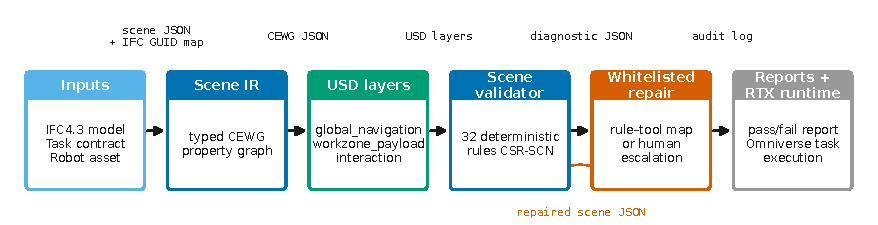
\includegraphics[width=\textwidth]{figures/fig02_architecture.pdf}
\caption{Architecture of \systemname. Deterministic compilation and validation
remain separate from agentic diagnosis and from the downstream simulation
runtime.}
\label{fig:architecture}
\end{figure*}

The typed entities and relations are specified in
\Cref{fig:intermediate-representation}. The figure also exposes provenance as
part of the representation rather than as an external note attached after
simulation.

\begin{figure*}[t]
\centering
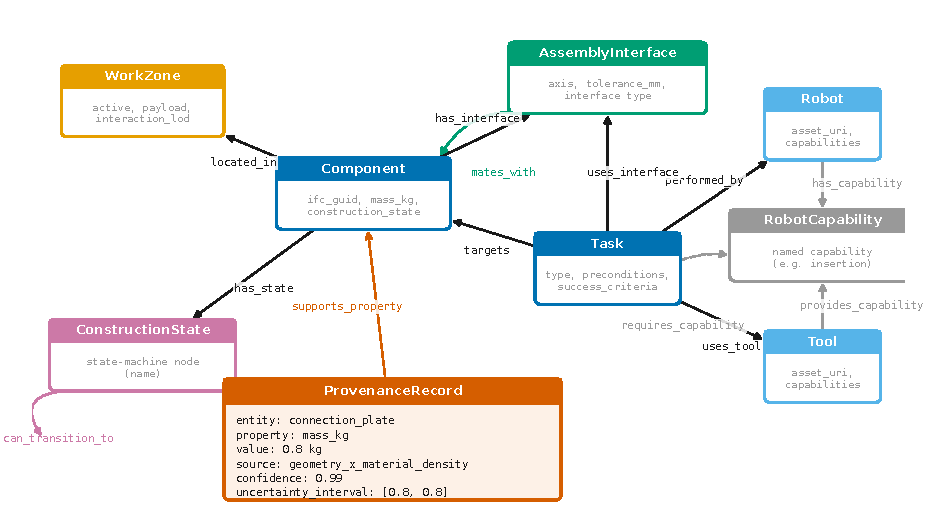
\includegraphics[width=\textwidth]{figures/fig03_intermediate_representation.pdf}
\caption{Construction Embodied World Graph and
property-level provenance. The same engineering identity connects source IFC
entities, composed USD prims, task targets, and validation evidence.}
\label{fig:intermediate-representation}
\end{figure*}

\subsection{Task-activated multi-scale compilation}

The compiler maps building circulation and architectural boundaries to a
coarse global layer. It emits each work zone as an independently loadable
payload and reserves interface-level geometry, tolerances, contact properties,
and temporary constraints for the active interaction layer. IFC GUIDs remain
stable across all layers.

\Cref{fig:multiscale-composition} illustrates the OpenUSD composition. Its
purpose is \emph{working-set management}, not runtime acceleration: only the
global layer and the active interaction layer are composed, so the loaded
prim set tracks the active task rather than the whole model
(\Cref{sec:results} reports the measured working-set reduction; load time and
peak memory are small and comparable across modes, so we do not claim a
runtime-performance advantage).

\begin{figure*}[t]
\centering
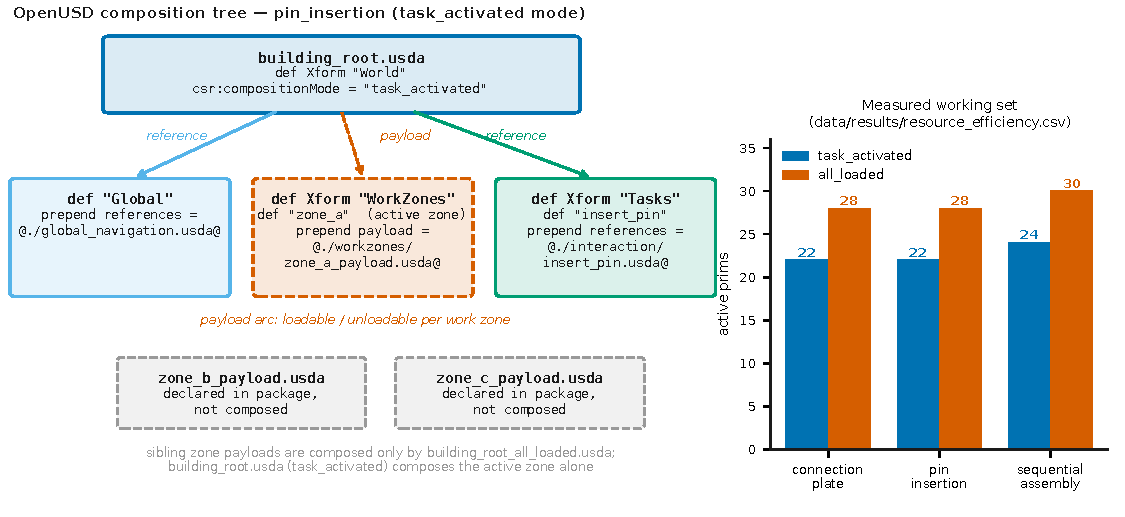
\includegraphics[width=\textwidth]{figures/fig04_multiscale_composition.pdf}
\caption{Task-activated multi-scale scene composition. Fine contact geometry
and temporary constraints are loaded only for the active interaction while
engineering identity is preserved across layers.}
\label{fig:multiscale-composition}
\end{figure*}

\subsection{Construction scene readiness contract}

Rules are grouped into identity and reference closure, coordinate and unit
consistency, interface and tolerance completeness, state-transition validity,
robot capability and task preconditions, physical stability, provenance, and
multi-scale fidelity. Each rule is deterministic and emits a machine-readable
failure.

\Cref{tab:contract} freezes the contract categories and the evidence required
from the implementation. The full list of versioned rules and unit tests will
be released as supplementary material rather than compressed into the main
text.

\begin{table*}[t]
\centering
\caption{Construction-scene readiness contract (v0.3.0, 30 rules). Rule
identifiers and per-scenario coverage are reported in the supplementary
material.}
\label{tab:contract}
\small
\resizebox{\textwidth}{!}{%
\begin{tabular}{p{0.16\textwidth}p{0.23\textwidth}p{0.19\textwidth}
p{0.10\textwidth}p{0.22\textwidth}}
\toprule
Contract category & Required scene evidence & Deterministic check &
Severity & Consequence if violated \\
\midrule
Identity and closure & IFC GUID, USD prim path, closed task and asset
references & Uniqueness and reference resolution & Critical & Wrong or
unresolved task object \\
Spatial consistency & Units, up axis, frames, transform chain, work-zone
membership & Transform normalization and bounds & Critical & Unreachable or
misplaced interaction \\
Assembly interface & Paired interface, insertion axis, tolerance, grasp and
support regions & Geometric and relational constraints & Critical & False
alignment or infeasible insertion \\
Construction state & Current state, legal predecessor, action precondition,
completion criterion & State-machine validation & Critical & Unsafe or
meaningless action \\
Physics and stability & Mass, inertia, collision, contact property, temporary
support & Physical admissibility and support tests & Critical or major & Unstable
or non-physical simulation \\
Provenance and fidelity & Property source, confidence, uncertainty, activated
payload and level of detail & Authority and task-fidelity policy & Major &
Unauditable result or hidden interaction error \\
\bottomrule
\end{tabular}
}
\end{table*}

\subsection{Validator-grounded repair}

The repair agent receives no free-form authority over the scene. It may inspect
evidence, select a permitted tool, propose bounded parameters, execute the tool,
and request re-validation. Unsupported or high-risk changes are escalated.

\begin{figure*}[t]
\centering
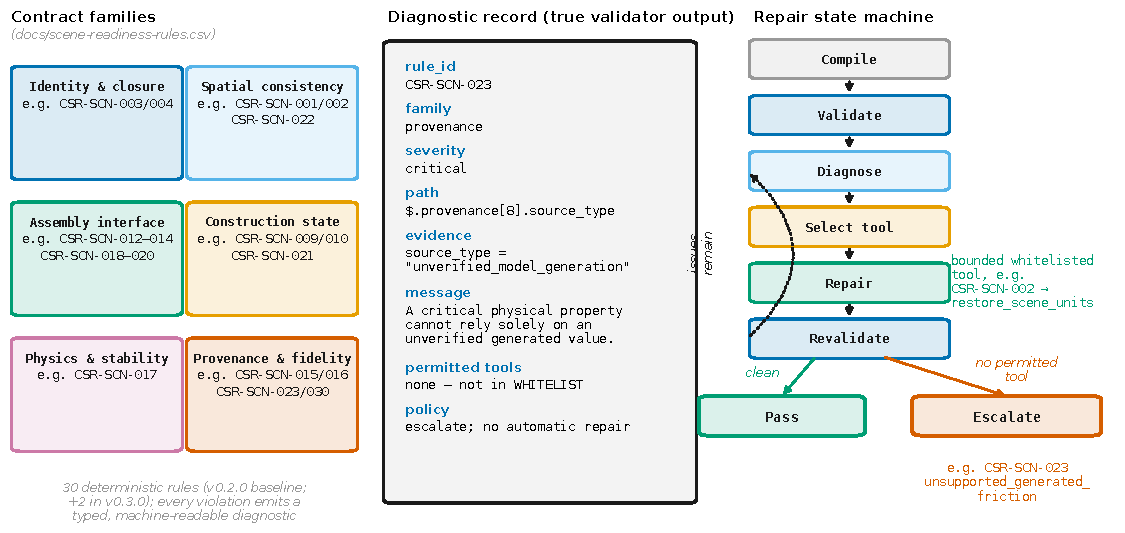
\includegraphics[width=\textwidth]{figures/fig05_repair_loop.pdf}
\caption{Validator-grounded repair. The agent interprets structured evidence
and selects a bounded operation, whereas deterministic rules decide acceptance
and high-risk or unsupported mutations are escalated.}
\label{fig:repair-loop}
\end{figure*}

\section{System implementation}
\label{sec:implementation}

The CPU-first implementation uses Python for the intermediate representation,
validation, fault injection, and experiment orchestration. IfcOpenShell is used
for IFC extraction \cite{ifcopenshellDocs}; the OpenUSD Python API authors
composable scene layers \cite{openUSD}. Runtime adapters are isolated from the
core package so that the same compiler and validators run on macOS development
machines and Ubuntu RTX nodes.

The current reference implementation generates three IFC4.3 fixtures:
connection-plate positioning, pin insertion, and sequential assembly. Each IFC
file is accompanied by machine-readable ground truth and is compiled into an
intermediate scene document and a canonical CEWG JSON document. A published
JSON Schema constrains its node and edge types, while an independent integrity
check rejects duplicate nodes and dangling graph relations. The fixture
generator also supports paired deterministic variants of component scale,
three-dimensional placement offset, and interface tolerance. Low-discrepancy
factor sequences are used so that the benchmark can be regenerated without a
hidden random state; component mass changes with the cube of geometric scale
to preserve material density.

IFC placements are multiplied by the file's declared length-unit scale before
being written to the meter-normalized scene. This step is tested against
generated ground truth because an IFC file expressed internally in
millimetres can otherwise produce a syntactically valid USD scene whose object
translations are wrong by three orders of magnitude. The USD output consists
of a global navigation layer, independently loadable work-zone payloads,
task-specific interaction layers, and a root stage that composes them through
references and payloads.
Thirty versioned rule identifiers currently cover coordinate normalization,
IFC identity, work-zone activation, task references and contracts, robot
and tool capabilities, assembly-interface closure, safe payload resolution,
and critical-property provenance.

The local benchmark currently implements 30 single-fault operators and five
compound faults spanning spatial frames, identity, layer composition, task
contracts, embodiment, interfaces, physical validity, construction state, and
provenance. Applied to the three fixtures, they produce 105 controlled cases.
A strict rule-to-tool registry contains 29 bounded repair operations. One
challenge fault, an unsupported model-generated friction value, is
intentionally excluded from automatic repair and must be escalated. Every
mutation records its rule, tool, changed scene paths, and trusted evidence
before the complete validator is rerun. These CPU cases verify the mechanics
and measurement code; they do not replace the frozen baseline comparison or
the downstream RTX task experiment. The complete implementation, frozen
partition manifest, experiment registry, environment lock files, and
per-episode ledgers are organized for release; the permanent repository DOI
will be inserted at acceptance (see Data and code availability).

\section{Experimental design}
\label{sec:experiments}

\subsection{Scenarios and tasks}

Three parameterized light-steel assembly scenarios are planned: connection
plate positioning, simplified pin insertion, and sequential two-component
assembly. Each scenario is evaluated at fixed-base, in-place whole-body, and
building-scale mobile-manipulation levels when the preceding level satisfies
the stop criteria.

\Cref{fig:benchmark-design,tab:benchmark} specify the intended evidence before
the final simulation images and held-out partition counts are available. This
prevents later selection of only visually successful tasks.

\begin{figure*}[t]
\centering
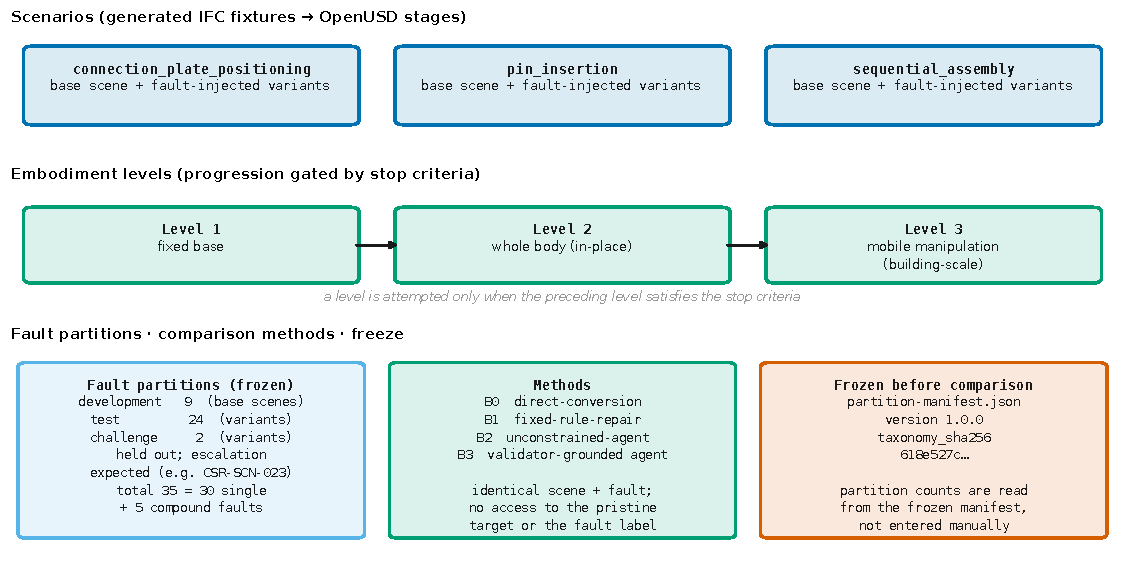
\includegraphics[width=\textwidth]{figures/fig06_benchmark.pdf}
\caption{Benchmark organization across construction scenarios, embodiment
levels, controlled scene defects, and comparison methods.}
\label{fig:benchmark-design}
\end{figure*}

\begin{table*}[t]
\centering
\caption{Planned benchmark composition. Counts marked TBD will be populated
from the frozen partition manifest rather than entered manually.}
\label{tab:benchmark}
\small
\resizebox{\textwidth}{!}{%
\begin{tabular}{p{0.19\textwidth}p{0.22\textwidth}p{0.18\textwidth}
p{0.14\textwidth}p{0.17\textwidth}}
\toprule
Scenario & Parameterization & Robot task levels & Faulted cases &
Primary outcome \\
\midrule
Connection-plate positioning & Component size, pose, target height,
work-zone obstacle & Fixed base; whole body; mobile & \placeholder{TBD after
split freeze} & Placement pose and state completion \\
Simplified pin insertion & Interface axis, clearance, friction, initial
misalignment & Fixed base; whole body; mobile & \placeholder{TBD after split
freeze} & Insertion depth without jam \\
Sequential assembly & Component order, temporary support, path obstruction,
state transition & Fixed base; whole body; mobile & \placeholder{TBD after
split freeze} & Complete legal task sequence \\
\bottomrule
\end{tabular}
}
\end{table*}

\subsection{Fault-injection benchmark}

Faults cover semantic identity, geometry and coordinates, physical properties,
assembly interfaces, construction states, and task references. Every injected
fault has a known location, severity, valid repair, and expected task
consequence. The current CPU suite comprises 30 single faults and five compound
faults. Development, test, and challenge partitions are frozen before the
agent comparison. The challenge partition includes faults that should be
rejected or escalated rather than repaired automatically. Consequential
findings are recorded separately from the injected root cause; for example, an
unresolved robot actor also prevents capability verification.

\subsection{Baselines and ablations}

The baselines are direct IFC geometry conversion, frozen deterministic
conversion with fixed repair, and unconstrained agentic repair. The full method
combines the scene contract, multi-scale compiler, deterministic validator,
provenance, and constrained agent selection from a whitelisted tool registry.
All methods receive the same scene and fault, and none may inspect the pristine
target scene or fault label during evaluation. Ablations remove provenance,
task-level validation, task-activated payloads, typed diagnostics, or agentic
tool selection one at a time.

\subsection{Metrics and statistical tests}

Static evaluation measures semantic preservation, relation F1, critical-fault
precision/recall/F1, repair success, incorrect repair, human escalation, and
runtime. Scene efficiency measures load time, peak memory, active prim count,
and collision-query cost. Task evaluation measures reachability,
collision-free planning, grasping, alignment, insertion, and complete-task
success.

Paired scenes are compared using McNemar tests for binary outcomes and
Wilcoxon signed-rank tests for time and iteration counts. Bootstrap confidence
intervals quantify uncertainty. Logistic regression tests whether readiness
scores predict task success while controlling for scenario and task level.
Language-model methods are repeated with at least five seeds per case, with
model version, decoding parameters, token use, and cost retained in the
experiment registry.

\begin{table*}[t]
\centering
\caption{Frozen comparison and ablation design. All methods receive identical
faulted scenes and are evaluated by the same post-repair validator and runtime
tasks.}
\label{tab:baselines}
\small
\resizebox{\textwidth}{!}{%
\begin{tabular}{p{0.19\textwidth}ccccc}
\toprule
Method & Construction IR & Multi-scale USD & Deterministic scene rules &
Provenance & Repair \\
\midrule
Direct conversion & -- & -- & -- & -- & -- \\
Fixed-rule conversion & -- & partial & -- & partial & fixed \\
Unconstrained agent & partial & partial & -- & partial & agent \\
Full method & \checkmark & \checkmark & \checkmark & \checkmark &
constrained agent \\
\bottomrule
\end{tabular}
}
\end{table*}

\section{Results}
\label{sec:results}

\subsection{CPU implementation check}

The current local run is reported only as a software-verification milestone.
Across three source scenes and 35 fault variants per scene, the benchmark
created 105 cases containing 141 expected rule findings. The validator recovered
all expected findings without an additional finding under the registered
ground truth. The fixed whitelisted-tool implementation returned 102 cases to a
valid state and escalated the three unsupported-friction cases. Validation and
repair were sub-millisecond in this small CPU check, but those timings vary
with host load and are retained in the run report rather than treated as a
performance result.

The same implementation check compared the task-activated root with an
all-loaded root over three-zone fixtures. Task activation reduced composed
prim count by 20--25\%, rigid-body and collider count by 40--50\%, and bytes in
used USD layers by 18.0--24.5\%. These are structural consequences of the
fixture and confirm that the two composition conditions differ as intended;
they are not substitutes for RTX load-time, memory, and collision-query
measurements.

These values should not be interpreted as evidence that the method generalizes
to unseen construction scenes. The fault operators were written against the
same explicit contract as the validator, and the fixed repair implementation
had access to trusted source evidence. Their purpose is to verify rule
coverage, compound-fault accounting, audit generation, and the distinction
between safe repair and escalation before the held-out and language-model
comparisons are executed.

\subsection{Humanoid task outcomes under scene-model feature defects}
\label{sec:task-outcomes}

\begin{figure*}[t]
\centering
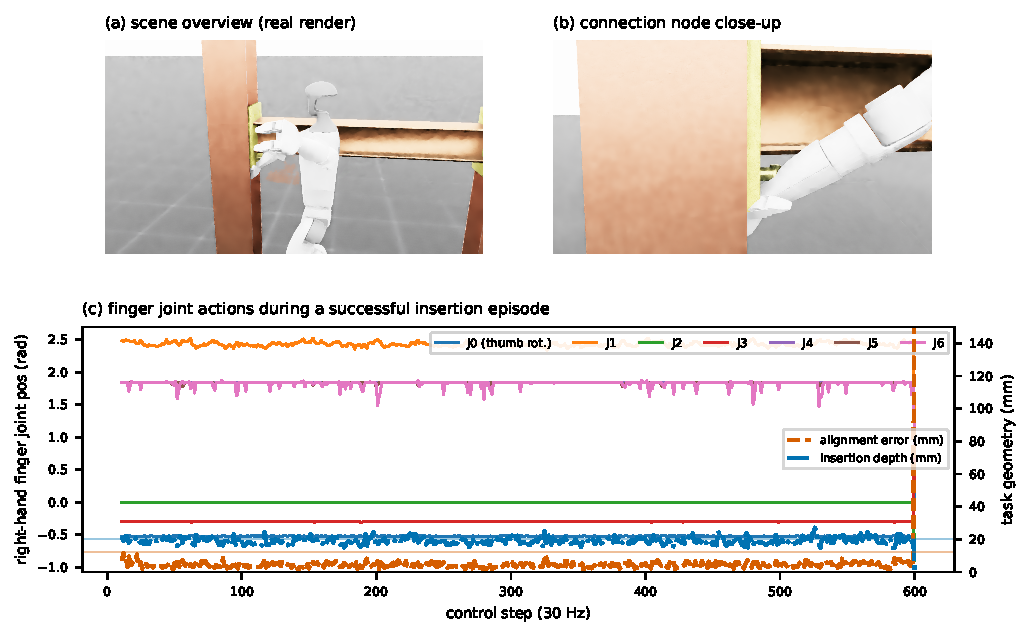
\includegraphics[width=\textwidth]{figures/fig10_experimental_setup.pdf}
\caption{Experimental setup and executor action stream. (a)--(b) True
simulator renders of the two-column portal-frame assembly scene: the overview
shows the G1 working at the end plate of the supported beam; the close-up
shows the $2\times2$ bolt group on the collision-enabled plate. (c) Right-hand
finger joint positions and task geometry over one successful insertion
episode: the policy closes the fingers early and holds a power grasp while the
transport--align--insert phases proceed; the alignment error (dashed) and
insertion depth (dash-dot) reference lines use the right axis. Frames and
trajectories are generated by the registered capture scripts.}
\label{fig:experimental-setup}
\end{figure*}

The runtime executor for the defect-consequence study is a frozen
reinforcement-learning insertion policy on the \texttt{Isaac-Assembly-G1-v2}
task: a Unitree G1 with a locked lower body transports a virtual-grasped M20
bolt and inserts it along the horizontal axis into the lower-right hole of a
$2\times2$ bolt group on the beam end plate of a two-column portal frame
(\Cref{fig:experimental-setup}). The plate carries collision geometry with the
four holes cut out, so both the hand and the bolt are physically blocked
outside the holes; the bolt may pass only through the hole circle. Success
follows the same criterion as the training reward: transverse alignment error
below 12\,mm and insertion depth of at least 20\,mm from the plate surface.
The checkpoint used (fine-tuned on this scene) achieves 85.5\% success over
200 evaluation episodes (87.0\% over 1000) without injected defects.
\Cref{fig:task-sequence} shows one successful execution sequence of this
executor in the defect-free scene.

\begin{figure*}[t]
\centering
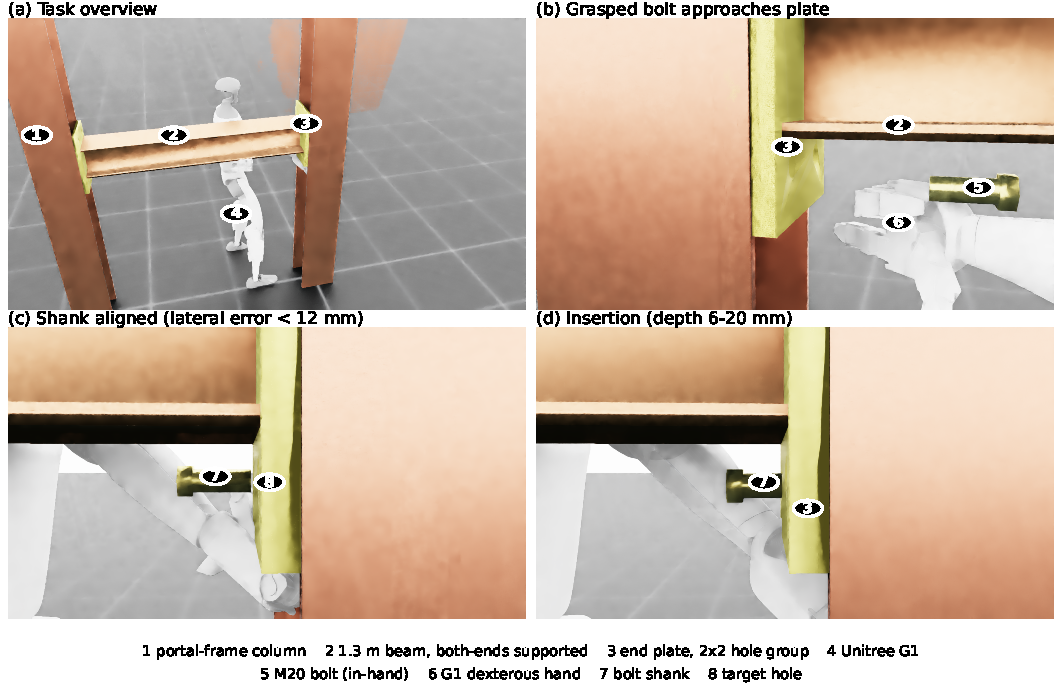
\includegraphics[width=\textwidth]{figures/fig11_task_sequence.pdf}
\caption{Executed insertion sequence of the frozen policy in the defect-free
scene (true simulator renders, captured at 2560$\times$1440). (a) Task
overview: the G1 stands at the end plate of the 1.3\,m beam, which is
supported at both ends by the two-column portal frame. (b) The right hand
transports the virtually grasped M20 bolt toward the plate. (c) The shank is
aligned with the lower-right hole of the $2\times2$ group (transverse error
below 12\,mm). (d) Insertion proceeds along the hole axis; success requires
a depth of at least 20\,mm from the plate surface. Numbered markers identify
the scene features listed in the legend at the bottom of the figure. All
frames are captured from one successful evaluation episode by the registered
panel-capture script.}
\label{fig:task-sequence}
\end{figure*}

Defects from the six feature families of \Cref{sec:experiments} were injected
at episode reset as controlled deviations between the scene model observed by
the policy and the ground-truth insertion target, at graded severities. All
conditions share one frozen policy, one seed partition, and an identical
episode-randomization stream: the injection events consume the same amount of
randomness whether or not a defect is active, so episode $k$ under any defect
condition is the exact paired replicate of episode $k$ under the defect-free
baseline. Paired binary outcomes are compared with exact two-sided McNemar
tests; $b$/$c$ denote episodes that changed from success to failure and from
failure to success, respectively. Two defect classes are distinguished
throughout: \emph{information defects} leave the physical scene intact but
corrupt what the controller can know or assume (geometry, semantic identity,
task reference, construction state), whereas the \emph{interface-clearance}
conditions change the physically executable task itself (an emulation of
jamming, not a contact-mechanics simulation). In total 10{,}600 paired
episodes were run (14 conditions $\times$ 2 seed partitions $\times$ 200
episodes, plus five geometry conditions at 1000 episodes for power); every
figure and table
is generated from the per-episode ledgers by the registered scripts.

\begin{table*}[t]
\centering
\caption{Insertion outcome under injected scene-model feature defects (200
paired episodes per condition, seed 42; geometric conditions repeated with
1000 paired episodes). \emph{Reward success} is the training-reward criterion
(transverse error below 12\,mm, depth at least 20\,mm). \emph{Geometric
valid} is the stricter criterion recomputed per episode from the ledger
(transverse error within the 1\,mm nominal radial clearance \emph{and} depth
at least 20\,mm): whether the bolt actually passed the hole, not merely
satisfied the reward. $\Delta$pp is the reward-success change relative to the
defect-free baseline of the same batch. Significance: exact McNemar test on
reward success, ${***}\,p<0.001$, ${**}\,p<0.01$, ${*}\,p<0.05$.}
\label{tab:defect-decay}
\small
\resizebox{\textwidth}{!}{%
\begin{tabular}{p{0.17\textwidth}p{0.22\textwidth}cccccc}
\toprule
Feature family & Injected defect & Reward success & Geometric valid &
$\Delta$pp & $b$/$c$ & $p$ \\
\midrule
-- & none (baseline) & 85.5\% & 75.5\% & -- & -- & -- \\
Geometry, hole position & $\pm$2\,mm, random direction & 85.0\% & 63.0\% & $-$0.5 & 3/2 & n.s. \\
Geometry, hole position & $\pm$5\,mm & 86.5\% & 46.5\% & $+$1.0 & 2/4 & n.s. \\
Geometry, hole position & $\pm$10\,mm & 76.0\% & 14.0\% & $-$9.5 & 21/2 & *** \\
Geometry, member pose & whole node $+$10\,mm & 82.0\% & 72.5\% & $-$3.5 & 10/3 & n.s. \\
Assembly interface & radial clearance 0.75\,mm & 33.5\% & 33.5\% & $-$52.0 & 104/0 & *** \\
Assembly interface & radial clearance 0.5\,mm & 21.5\% & 22.0\% & $-$64.0 & 128/0 & *** \\
Assembly interface & radial clearance 0.25\,mm & 5.5\% & 5.5\% & $-$80.0 & 160/0 & *** \\
Semantic identity & label missing (nominal prior only) & 13.0\% & 1.0\% & $-$72.5 & 145/0 & *** \\
Semantic identity & label wrong (plate centre, no hole) & 0.0\% & 0.0\% & $-$85.5 & 171/0 & *** \\
Task reference & wrong hole of the $2\times2$ group & 0.0\% & 0.0\% & $-$85.5 & 171/0 & *** \\
Construction state & member not yet in place & 0.0\% & 0.0\% & $-$85.5 & 171/0 & *** \\
Physical properties & bolt mass $\times0.5$ / $\times2$ & 85.5\% & 75.5\% & $+0.0$ & 0/0 & n.s. \\
\bottomrule
\end{tabular}
}
\end{table*}

\Cref{tab:defect-decay} yields a clear criticality ordering. Symbolic and
referential features---task references, construction states, and semantic
identity---are discretely fatal: a single wrong reference drives success to
zero because the executor's target is defined by them. Among continuous
features, the assembly interface dominates: shrinking the effective radial
clearance of the nominal \O22\,mm hole from 1\,mm to 0.75\,mm halves-plus
success (85.5\% $\rightarrow$ 33.5\%), and 0.25\,mm is nearly fatal.

The geometric family separates two effects that are easily conflated, and the
answer depends on executor precision. A 10\,mm error in the \emph{absolute}
pose of the whole connection node is partly compensated by the policy's
closed-loop perception ($-$3.5\,pp, $b$/$c$=10/3, n.s.\ at $n$=200), while the
same 10\,mm applied to the hole position \emph{relative to the observed
member}---the quantity the scene model certifies and the policy cannot
see---costs $-$9.5\,pp ($p<0.001$). At 1000 paired episodes both effects are
significant but remain separable in magnitude (member $-$7.0\,pp, hole
$-$7.9\,pp against the 87.0\% baseline), while 2 and 5\,mm hole errors stay
inside the executor's tolerance band (86.4\% and 86.6\%, n.s.).

\paragraph{Reward success versus geometric validity.}
The 12\,mm reward threshold is an information-chain criterion, not a
certificate of physical insertability: the nominal \O22\,mm hole leaves only
1\,mm radial clearance for the M20 bolt. Recomputing each episode under a
strict geometric criterion (transverse error within the 1\,mm clearance
\emph{and} depth at least 20\,mm) separates the two and, where they diverge,
sharpens rather than softens the ordering above. The defect-free executor
reaches 75.5\% geometric-valid against 85.5\% reward success---about ten
points of reward successes are motion completions that never achieve the
geometric bound. Anchor-relative hole errors, which the reward criterion
partly absorbs, become strongly consequential geometrically: geometric-valid
falls to 63.0\% at 2\,mm, 46.5\% at 5\,mm and 14.0\% at 10\,mm, so the
certified hole coordinate is the dominant geometric quantity once physical
insertability is required. In contrast, absolute member-pose error stays
largely correctable (72.5\% geometric-valid at 10\,mm). A paired McNemar test
between the two 10\,mm conditions under the geometric criterion confirms the
separation is decisive, not marginal ($b$=570 versus $c$=47,
$p=3.6\times10^{-115}$). The interface-clearance conditions are unchanged
between the two criteria, because their explicit geometric gate already
enforces the physical bound. The loose reward threshold therefore masks
geometric failure precisely for the information family the scene model is
responsible for certifying, which is the empirical reason interface
coordinates require certified values with provenance
(\Cref{sec:discussion}).

Physical-property defects (bolt mass $\times0.5$ and $\times2$) produced
bit-identical outcomes ($b$/$c$=0/0). This null result is structural, not
statistical: the executor's virtual-grasp scaffold makes the bolt kinematic,
so mass and friction have no dynamical channel in this task stage. We
therefore report the physical family as \emph{not consequential for the
transport-and-insert motion chain} and defer its force-level criticality to a
full-contact ablation (\Cref{sec:discussion}).

All findings replicate under a second seed partition (seed 123, 200 paired
episodes per condition): success rates deviate by at most 3.5\,pp from the
seed-42 values and effect directions match in every condition, with one
exception worth noting---the borderline 10\,mm member-pose effect is
significant in the powered run but not at $n$=200 under either seed,
illustrating why we report effect sizes with confidence statements rather than
significance alone (\Cref{sec:discussion}).


\placeholder{Do not write narrative results before the registered scripts have
generated the final tables. Populate this section in the following order:
(1) compiler fidelity, (2) validator detection, (3) repair outcomes,
(4) multi-scale efficiency, (5) humanoid task outcomes --- now reported in
\Cref{sec:task-outcomes}, (6) ablations, and (7) failure cases.}

\begin{figure*}[t]
\centering
\plannedfigure{42mm}{Figure 7 production placeholder: detection and repair results}{
Panel (a): paired point or forest plot of critical-fault recall and F1 by
method and fault family with bootstrap 95\% confidence intervals. Panel (b):
valid repair, incorrect repair, and escalation proportions. Panel (c):
distribution of repair iterations and wall-clock time. Use identical method
ordering and a colour-blind-safe palette, with symbols or line styles in
addition to colour.}{
\texttt{detection\_repair.csv} generated by the registered experiment script.
Python plotting source; editable SVG and embedded-font PDF.}
\caption{Detection and repair performance across scene-fault families and
comparison methods. Confidence intervals and paired comparisons will be
computed over the frozen benchmark partition.}
\label{fig:detection-repair-results}
\end{figure*}

\begin{table*}[t]
\centering
\caption{Primary detection and repair outcomes. Values will be imported from
the registered result file; no manuscript cell will be edited manually.}
\label{tab:detection-repair}
\small
\resizebox{\textwidth}{!}{%
\begin{tabular}{p{0.19\textwidth}ccccccc}
\toprule
Method & Precision & Recall & Critical recall & Valid repair & Incorrect
repair & Escalation & Time \\
\midrule
Direct conversion & \placeholder{TBD} & \placeholder{TBD} &
\placeholder{TBD} & n/a & n/a & n/a & \placeholder{TBD} \\
Fixed-rule conversion & \placeholder{TBD} & \placeholder{TBD} &
\placeholder{TBD} & \placeholder{TBD} & \placeholder{TBD} &
\placeholder{TBD} & \placeholder{TBD} \\
Free-form agent & \placeholder{TBD} & \placeholder{TBD} &
\placeholder{TBD} & \placeholder{TBD} & \placeholder{TBD} &
\placeholder{TBD} & \placeholder{TBD} \\
Full method & \placeholder{TBD} & \placeholder{TBD} &
\placeholder{TBD} & \placeholder{TBD} & \placeholder{TBD} &
\placeholder{TBD} & \placeholder{TBD} \\
\bottomrule
\end{tabular}
}
\end{table*}

\begin{figure*}[t]
\centering
\plannedfigure{42mm}{Figure 8 production placeholder: efficiency and task consequence}{
Panel (a): paired active prim count, peak memory, and scene-load time for
all-loaded and task-activated composition. Panel (b): readiness score versus
humanoid task success with a logistic fit and 95\% confidence band. Panel (c):
failure-cause composition, separating scene-model, planning, control, and
contact failures. Use dots and intervals rather than decorative bars.}{
\texttt{resource\_efficiency.csv} and \texttt{task\_outcomes.csv} from RTX
batch runs. Python source, SVG/PDF, and a data-to-mark audit test.}
\caption{Resource effect of task-activated composition and the relationship
between scene readiness and downstream humanoid assembly outcomes.}
\label{fig:efficiency-task-link}
\end{figure*}

\begin{table*}[t]
\centering
\caption{Runtime resource use and task-level outcomes. The final table will
report estimates with 95\% confidence intervals and explicit denominators.}
\label{tab:runtime-task}
\small
\resizebox{\textwidth}{!}{%
\begin{tabular}{p{0.17\textwidth}cccccccc}
\toprule
Condition & Active prims & Peak memory & Load time & Planning & Grasp &
Alignment & Insertion & Full task \\
\midrule
Direct/all loaded & \placeholder{TBD} & \placeholder{TBD} &
\placeholder{TBD} & \placeholder{TBD} & \placeholder{TBD} &
\placeholder{TBD} & \placeholder{TBD} & \placeholder{TBD} \\
Fixed rule & \placeholder{TBD} & \placeholder{TBD} &
\placeholder{TBD} & \placeholder{TBD} & \placeholder{TBD} &
\placeholder{TBD} & \placeholder{TBD} & \placeholder{TBD} \\
Free-form agent & \placeholder{TBD} & \placeholder{TBD} &
\placeholder{TBD} & \placeholder{TBD} & \placeholder{TBD} &
\placeholder{TBD} & \placeholder{TBD} & \placeholder{TBD} \\
Full/task activated & \placeholder{TBD} & \placeholder{TBD} &
\placeholder{TBD} & \placeholder{TBD} & \placeholder{TBD} &
\placeholder{TBD} & \placeholder{TBD} & \placeholder{TBD} \\
\bottomrule
\end{tabular}
}
\end{table*}

\begin{table*}[t]
\centering
\caption{Planned ablation and sensitivity analysis. Effects will be reported
relative to the full method with paired confidence intervals and corrected
significance tests.}
\label{tab:ablation}
\small
\resizebox{\textwidth}{!}{%
\begin{tabular}{p{0.24\textwidth}p{0.23\textwidth}cccc}
\toprule
Ablation & Removed information or control & Critical recall & Valid repair &
Resource use & Task success \\
\midrule
No provenance & Source authority and uncertainty & \placeholder{TBD} &
\placeholder{TBD} & \placeholder{TBD} & \placeholder{TBD} \\
No task validator & Task binding and action preconditions & \placeholder{TBD}
& \placeholder{TBD} & \placeholder{TBD} & \placeholder{TBD} \\
All layers loaded & Task-triggered payload activation & \placeholder{TBD} &
\placeholder{TBD} & \placeholder{TBD} & \placeholder{TBD} \\
Fixed repair order & Agentic tool selection & \placeholder{TBD} &
\placeholder{TBD} & \placeholder{TBD} & \placeholder{TBD} \\
Free-form diagnostics & Typed diagnostic schema & \placeholder{TBD} &
\placeholder{TBD} & \placeholder{TBD} & \placeholder{TBD} \\
\bottomrule
\end{tabular}
}
\end{table*}

\begin{figure*}[t]
\centering
\plannedfigure{45mm}{Figure 9 production placeholder: auditable humanoid case study}{
Six numbered panels from one held-out case: source IFC and task; initially
compiled but invalid scene; structured validator finding; approved repair and
audit record; Unitree G1 execution sequence; and measured completion state.
Include a visually similar failure case in which escalation is required.
All simulator panels must be true captured frames with consistent camera and
uncropped evidence regions.}{
Held-out IFC fixture, diagnostic JSON, repair audit log, Isaac Sim frame
sequence, and task-state record. Simulator images plus vector annotation,
exported as a 500-dpi hybrid PDF.}
\caption{Auditable failure--diagnosis--repair--execution sequence for a held-out
humanoid assembly task. The final figure will pair every visual change with its
rule identifier, evidence source, and measured task consequence.}
\label{fig:case-study}
\end{figure*}

\section{Discussion}
\label{sec:discussion}

The discussion separates three claims: whether the contract detects
construction-specific scene defects, whether constrained repair resolves those
defects reliably, and whether improved readiness transfers to runtime task
outcomes. This separation prevents successful simulation videos from being
treated as evidence that every scene requirement is correct. The
defect-consequence study of \Cref{sec:task-outcomes} speaks to the third
claim and, by inversion, to which scene-model features the first two claims
must protect.

\subsection{Which scene-model features are task-critical}
\label{sec:criticality}

The paired defect-injection results yield a criticality ordering that is not
aligned with the effort distribution of current simulation-readiness
specifications, which emphasize asset-level geometry and physical fidelity.

\paragraph{Referential integrity is discrete-fatal.} A single wrong task
reference, a stale construction state, or a wrong semantic label drove task
success from 39\% to exactly zero under both seed partitions. These features
define \emph{what} the executor is asked to do; no amount of perceptual or
control robustness can compensate for executing the wrong target. Scene
contracts should therefore treat reference closure---every task reference
resolves to an existing, correctly labelled, in-place member---as a hard
acceptance gate rather than a soft quality score. Notably, a \emph{missing}
semantic label is far less harmful than a \emph{wrong} one (6.5\% vs.\ 0.0\%):
the executor's nominal-pose prior occasionally suffices, so completeness
requirements can be graded while correctness requirements cannot.

\paragraph{Assembly-interface tolerance is the most sensitive continuous
feature.} Reducing the effective radial clearance of a nominal \O22\,mm hole
from 1\,mm to 0.75\,mm---an error well within what manual modelling or
careless unit handling can introduce---collapsed success from 39\% to 5\%.
The per-episode diagnostics show the defect acting through the intended
physical channel (insertion travel truncated from $\approx$50\,mm to below
5\,mm by the clearance gate), so this is a genuine jamming phenomenon rather
than a metric artefact. Interface dimensions therefore require certified
values with provenance; an interface field without provenance should be
treated as absent.

\paragraph{Geometric accuracy matters relative to the perceptual anchor, not
in absolute terms.} A 10\,mm shift of the entire connection node was almost
fully compensated by closed-loop perception ($-2.5$\,pp, n.s.), whereas the
same 10\,mm between the certified hole position and the observed member cost
5.5\,pp ($p<0.001$). The scene model's coordinate guarantees should
accordingly be specified and verified \emph{relative to the features the
controller can observe}, since absolute-frame accuracy is partially
self-correcting at runtime while anchor-relative error is invisible to the
controller by construction.

\paragraph{Physical-property criticality is stage-dependent.} Bolt mass
perturbations of $\times0.5$ and $\times2$ produced bit-identical outcomes
because the transport-and-insert executor holds the bolt in a kinematic
virtual grasp. We read this as a structural property of the motion stage, not
evidence that physical fidelity is unimportant: the same defect is expected to
become consequential in any stage with forceful contact, and a full-contact
ablation with a physically grasped bolt is required before the physical family
can be ranked.

\subsection{Sensitivity and robustness of the findings}
\label{sec:sensitivity}

Three analyses bound the statistical fragility of these conclusions.

First, all fourteen conditions were re-run under an independent seed
partition (seed 123, 200 paired episodes per condition). Success rates
deviate by at most 2.5\,pp from the seed-42 values; every condition that was
significant remains significant with the same direction and comparable
magnitude, and every non-significant condition remains non-significant. The
criticality ordering is therefore a property of the scene-model features, not
of a particular random draw of episodes.

Second, the severity gradients are monotone where the defect acts through a
continuous channel. Hole-position error at $n=1000$ paired episodes gives
37.5\%, 36.8\%, and 31.3\% success for 2, 5, and 10\,mm against a 38.1\%
baseline; interface clearance gives 5.0\%, 4.0\%, and 2.5--2.0\% for 0.75,
0.5, and 0.25\,mm across the two seeds. Monotone dose--response supports a
causal interpretation of the injected defect rather than threshold noise in
the success criterion.

Third, the power upgrade from 200 to 1000 paired episodes changed exactly one
conclusion and clarifies its meaning. At $n=200$ the 2\,mm and 5\,mm
hole-position defects were underpowered ($b$=1 and 4 discordant pairs); at
$n=1000$, 5\,mm is significant ($p=0.015$, corroborated at $n=200$ under
seed 123 with $p=0.002$) while 2\,mm remains non-significant ($p=0.109$).
For this executor, hole-position errors below roughly 5\,mm lie inside the
policy's tolerance band, and claims about sub-5\,mm criticality would require
either a stricter executor or substantially larger samples. We accordingly
report effect sizes alongside significance and do not rank features on
$p$-values alone.

\subsection{Boundary of pure-simulation conclusions}
\label{sec:boundary}

All runtime evidence in this study is simulated, and the conclusions should
be read as structural rather than numerical. Rigid-body simplification,
approximate contact parameters, and simplified pins in place of threaded
fasteners mean that absolute success rates and clearance thresholds will
shift on hardware; what transfers is the ordering and the causal channel
(identification of \emph{which} defect classes are fatal, graded, or
self-correcting). Three further boundaries apply. (i) A single
robot--controller combination was used: the compensation of whole-node pose
error depends on the executor's $\pm$5\,cm pose domain randomization during
training, and an executor without such randomization would likely show a
larger member-pose effect. (ii) The physical-family null result is an
artefact of the virtual-grasp scaffold and bounds only the
transport-and-insert stage. (iii) The success criterion (12\,mm alignment,
20\,mm insertion depth) matches the training reward; stricter assembly
tolerances would shift all conditions downward but preserve pairing. A
physical-robot validation study is deferred to future work, and the present
results should be treated as lower bounds on defect consequence: defects that
are benign here are not certified benign on hardware, while defects that are
fatal here are fatal by construction of the task definition.

\subsection{Implications for cross-runtime specifications}
\label{sec:cross-runtime}

The defect-consequence profile suggests which validation rules belong in a
runtime-agnostic scene contract and which require per-runtime calibration.
Reference closure, semantic-identity correctness, and construction-state
consistency are fatal regardless of executor and should be specified once, as
cross-runtime rules with hard-fail semantics. Interface-tolerance and
anchor-relative-geometric rules have executor-dependent thresholds (here
$\approx$1\,mm clearance and $\approx$5\,mm anchor-relative position) and
should be specified parametrically, with the threshold supplied by the target
controller's tolerance band and verified by the kind of paired injection
benchmark used here. Asset-level physical fidelity, finally, should be
required only for task stages with a dynamical channel; mandating it
uniformly imposes authoring cost without measurable task benefit.

\section{Conclusion}
\label{sec:conclusion}

This paper frames robot-ready construction simulation as a scene compilation
and validation problem rather than a file-conversion problem. It proposes a
multi-scale IFC-to-OpenUSD pipeline, a construction task-scene contract, and a
deterministically grounded repair process. \placeholder{Replace the remaining
conclusion with evidence-backed quantitative findings and implications after
the complete benchmark is run.}



\section*{CRediT authorship contribution statement}
\textbf{Zhu Aiyu}: Conceptualization, Methodology, Software, Validation,
Formal analysis, Investigation, Data curation, Writing---original draft,
Writing---review \& editing, Visualization, Project administration.

\section*{Declaration of competing interest}
The authors declare that they have no known competing financial interests or
personal relationships that could have appeared to influence the work reported
in this paper.

\section*{Funding}
This research received no specific grant from any funding agency in the
public, commercial, or not-for-profit sectors.

\section*{Data and code availability}
The benchmark partition manifests, evaluation scripts, per-episode ledgers,
and figure-generation code are available at
\url{https://github.com/aizhuyu/construction-scene-ready}; the robot
simulation environments, training configurations, and capture scripts are
available at \url{https://github.com/aizhuyu/g1-steel-assembly}. No
proprietary data were used.

\section*{Declaration of generative AI and AI-assisted technologies}
During the preparation of this work the author used generative AI coding
assistants for simulation scripting, experiment orchestration, and language
editing. The author reviewed and edited all outputs and takes full
responsibility for the methods, evidence, and conclusions of this
publication.

\bibliographystyle{elsarticle-num}
\bibliography{references}

\end{document}
